\documentclass[]{IEEEtran}

\title{Sparse Matrix Transposition for GPUs}
\author{Massimiliano Incudini - VR433300\\Michele Penzo - VR439232}

\usepackage{graphicx}
\usepackage[export]{adjustbox}
\usepackage[italian]{babel}
\usepackage{dirtree}
\usepackage{hyperref}


\begin{document}
\maketitle

\begin{abstract}
	L'obiettivo principale di questo progetto è stato quello di implementare alcune metodologie proposte per effettuare \textit{Sparse Matrix Transposition} su \textit{Gpu}.
	Sono stati analizzati alcuni algoritmi, descritti in sezione~\ref{metodologie}, partendo dall'algoritmo seriale, passando a cuSPARSE per finire con l'implementazione degli algoritmi descritti in~\cite{parallelTrans}.
	Infine vengono esposti i risultati e tratte le conclusioni.
\end{abstract}


\section{Introduzione}
\label{introduzione}
	% problema e motivazioni
	Sempre più applicazioni computazionali in ambito scientifico necessitano di algoritmi che compiano operazioni che si possano applicare su matrici sparse. Si parla di semplici operazioni di algebra lineare, di moltiplicazione o di calcolo della trasposta come in questo caso.\newline
	Il problema analizzato, quello della trasposizione di matrici, si presta bene al calcolo parallelo per aumentarne l'efficienza. Verranno quindi mostrate le basi per la rappresentazione, i problemi riscontrati durante lo sviluppo e analizzati alcuni algoritmi per il calcolo su \textit{Gpu}.\newline


\section{Rappresentazione delle matrici}
\label{rappresentazione}
	Una matrice sparsa non è altro che una matrice i cui valori sono per la maggior parte uguali a zero. La matrice in formato classico necessita di una quantità di memoria minima di $ m $x$ n $ elementi, ma essendo l'obiettivo quello di lavorare su matrici sparse non è stato necessario e utile memorizzare la matrice in formato denso.\newline
	Per rappresentare in modo efficace le matrici sparse senza troppo utilizzo di memoria sono state quindi introdotte ed utilizzate delle forme di rappresentazione matriciale che permettono il salvataggio di dati utilizzando quantitativi di memoria inferiori.\newline
	Di seguito vengono spiegate le due metodologie da noi utilizzate.
	
	\subsection{Csr}
	\label{csr}
	Il \textit{compressed sparse row} è una rappresentazione di una matrice $ M $ basata su tre array monodimensionali, che rispettivamente contengono:
	\begin{enumerate}
		\item \textit{V}: i valori \textit{nnz},
		\item \textit{COL\_INDEX}: gli indici delle colonne dove si trovano gli elementi \textit{nnz},
		\item \textit{ROW\_INDEX}: ha un elemento per ogni riga della matrice e rappresenta l'indice in $ V $ dove comincia la riga data.
	\end{enumerate}
	I primi due array sono di dimensione \textit{nnz}, mentre il terzo array è al massimo di dimensione $ m $.
	
	\subsection{Csc}
	\label{csc}
 	Questa metodologia per la rappresentazione è simile alla sopra citata \textit{Csr}, a differenza che i valori vengono letti prima per colonna. Di conseguenza, un indice di riga viene memorizzato per ogni valore e i puntatori di colonna vengono memorizzati.
 	
	\subsection{Da Csr a Csc}
	\label{csr-to-csc}
 	Per il problema della trasposta di matrice è stato quindi utile introdurre entrambe le rappresentazioni. Infatti, ogni algoritmo  descritto in sezione~\ref{metodologie}, necessita di sei array per effettuare il calcolo della trasposta e ritornare l'output in modo corretto. Abbiamo quindi:
 	\begin{itemize}
 		\item in input il formato \textit{Csr}: csrRowPtr, csrColIdx, csrVal;
 		\item in output il formato \textit{Csc}: cscColPtr, cscRowIdx, cscVal.	
 	\end{itemize}
 	In base a come vengono create le matrici, se in modo casuale oppure se lette da file, vengono effettutate delle operazioni preliminari descritte dalla procedure in sezione~\ref{procedure} che portano ad ottenere gli array in input e in output nel formato corretto per effettuarne il controllo di correttezza.\newline
	
	% TODO disegnino fatto meglio
	\begin{figure}[h!]
		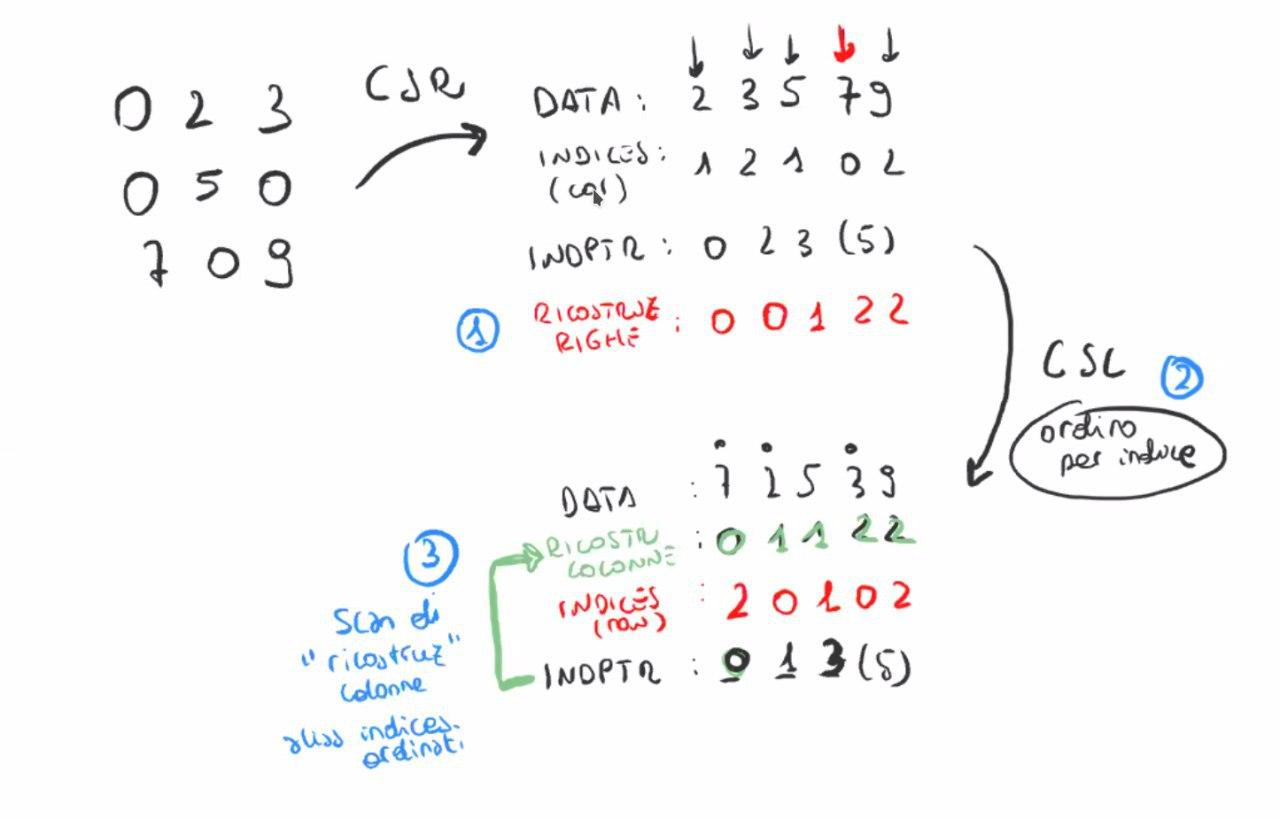
\includegraphics[scale=0.25]{figures/csr-to-csc.jpg}
		\caption{Esempio di trasformazione da formato Csr a Csc.}
	\end{figure}

	
\section{Struttura dell'implementazione} 
\label{struttura}
	L'implementazione è stata sviluppata utilizzando come supporto il tool \textit{Git}. È stata creata una repository, descritta nella sezione successiva, per poter controllare in modo efficiente lo svilupparsi del progetto. Tutti i test sono stati effettutati sulle macchine locali e sul server Cuda01.
	% TODO sisteamre newpage
	\newpage
	\subsection{Struttura delle directory}
	La struttura delle direcotry è rispecchiata nel seguente schema:
	\dirtree{%
		.1 repository.
			.2 doc.
				.3 {report\_aa.$ * $}.				
			.2 code.
				.3 {matrices}.
					.4 {$ *$.mtx }.
				.3 {include}.
					.4 {matrix.hh}.
					.4 {procedures.hh}.
					.4 {Timer.$ * $}.
					.4 {transposer.hh}.
					.4 {utilities.hh}.
				.3 {src}.
					.4 {all cuda\_procedures }.
					.4 {transposer.cu}.
					.4 {main.cu}.
				.3 {test}.	
					.4 {test\_main.cu}.
				.3 Makefile.			
			.2 README.md.
	}

	

	\subsection{Test delle componenti}	
	% singole componenti
	
	\subsection{Applicativo finale}
	% più matrici testate assieme

\section{Metodologie analizzate}
\label{metodologie}
	In questa sezione vengono spiegate ed evidenziate le differenze tra le varie metodologie analizzate. 
		
	\subsection{Trasposta seriale}
	La prima metodologia descritta è quella seriale. Sempre a partire dalla rappresentazione in formato \textit{csr} della matrice iniziale l'algoritmo crea un array di elementi, dove per ogni colonna della matrice analizzata conta quanti elementi \textbf{nnz} ci sono. Possiamo definire questo array come un istogramma delle frequenze degli elementi delle colonne. Viene quindi applicato un algoritmo seriale di \textit{prefix\_sum} su questo array, che conterrà ora i valori corretti di \textbf{cscColPtr}. Infine gli indici di riga e i valori nel nuovo formato \textit{csc} vengono sistemati.\newline
	Questa implementazione servirà come base sulla quale verranno eseguiti i controlli degli algoritmi successivamente implementati.
	
	\subsection{Nvidia cuSPARSE}
	Questo toolkit è implementato all'interno nelle librerie NVIDIA CUDA runtime. Le routine delle librerie vengono utilizzate per le operazioni tra vettori e matrici che sono rappresentate tramite diversi formati. Inoltre mette a disposione operazioni che permettono la conversione attraverso diverse rappresentazioni di matrici, ed inoltre la compressione in formato \textit{csr} che è una delle più usate quando si vuole rappresentare matrici sparse in modo efficiente.\newline	
	Il codice è stato sviluppato basandosi su due versioni di cuSPARSE a causa delle Gpu utilizzate. In fase di compilazione viene quindi controllata la versione usata: $ 9 $ o $ 10 $.\newline
	Nel caso in cui la versione usata sia la $ 10 $ vengono svolti alcuni ulteriori passi, viene effettuata l'allocazione dello spazio necessario e del buffer per il calcolo della trasposta. Per quanto riguarda la versione $ 9 $ invece questi passi non sono necessari.\newline
	Infine viene chiamata la procedura che effettua il calcolo della trasposta. \newline
	Le procedure chiamate sono diverse in base alla funzione. Nel primo caso viene chiamata \textbf{cusparseScsr2csc}, mentre nel secondo caso \textbf{cusparseCsr2cscEx2}. Quest'ultima richiede come parametro anche l'algoritmo che viene utilizzato all'interno della procedura.\newline
	Dopo essere state eseguite entrambe ritornano i valori ottenuti tramite un'altro formato, \textit{csc}, che ne esprime la rappresentazione tramite valori come csrColIdx, cscVal, cscColPtr, cscRowIdx. Infine viene controllata la correttezza e i tempi rispetto alle altre implementazioni.

	\subsection{ScanTrans}
	
	
	\subsection{MergeTrans}
	

\section{Procedure}
\label{procedure}
% tutte le versioni x2 e x3

	\subsection{Index to pointers}
	\label{idx-to-pnt}
	
	\subsection{Pointers to index}
	\label{pnt-to-idx}
	
	\subsection{Merge}
	\label{merge}
		\subsubsection{Segmented Sort}	

		\subsubsection{Merge big}	

		\subsubsection{Merge small}	
		
	\subsection{Sort}
	\label{sort}
	

\section{Benchmark}
\label{benchmark}
	\subsection{Matrici piene}
	
	\subsection{Matrici sparse casuali}

	\subsection{Dataset utilizzato}
	% dataset? matrici come sono state implementate?
	
	
\section{Risultati}
\label{risultati}
	% file csv
	% tabellone 

\section{Conclusioni}
\label{conclusioni}
	% cosa migliorare?


\bibliographystyle{IEEEtran}
\bibliography{biblio}

%\appendix
%Se non avete abbastanza spazio, potete inserire le figure delle EFSM in una  pagina extra, appendice. Un esempio di come potete fare solo le Figure~\ref{fig:grande}, \ref{fig:piccola1}, \ref{fig:piccola2}.

\end{document}